% !TEX program = xelatex
\documentclass[a4paper]{article}
\usepackage{amsthm}
\usepackage{amssymb}
\usepackage{bm}
\usepackage{mathtools}
\usepackage[x11names]{xcolor}
\usepackage{xparse}
\usepackage{fontspec}
\usepackage{unicode-math}
\setromanfont{DovesType-Regular.otf}
\setsansfont{Andika}
\setmathfont{Asana Math}[Scale=1]

% \usepackage{pstricks}
\usepackage{varwidth}
\usepackage{siunitx}
\usepackage{graphicx}
\usepackage[margin=2.5cm,top=3cm]{geometry}
\usepackage[most]{tcolorbox}
\usepackage{pgfplots}
\pgfplotsset{compat=newest}
\tcbuselibrary{skins,xparse,poster,breakable}
% \usetikzlibrary{fadings}
\usetikzlibrary{calc, plotmarks, shapes, shapes.geometric, positioning, angles, intersections, quotes, through, patterns, turtle, arrows.meta}
\usetikzlibrary{decorations.markings,backgrounds}
% \usepackage{etoolbox}
% \usepackage{tkz-euclide}
% \usepackage{xlop}
% \newcommand\hole[2]{#1}  % for use with xlop
\pagenumbering{gobble}
%%%%%%%%%%%%%%%%%%%%%%%%%%%%%%%%%%%%%%%%%%%%%%%%%%%%%%%%%
\newcommand\markangle[9]{% origin X Y radius radiusmark mark colour opacity
%  % fill red circle offset-from-centre
  \begin{scope}
    \path[clip] (#1) -- (#2) -- (#3);
    \fill[color=#7,fill opacity=#8,draw=black,name path global=pcircle]  % global declaration required otherwise pcircle is not seen by the `named intersections=' lines below.
    (#1) circle (#4);
  \end{scope}
  % middle calculation
  \path[name path=line one] (#1) -- (#2);
  \path[name path=line two] (#1) -- (#3);
  \path[%
  name intersections={of=line one and pcircle, by={inter one}},
  name intersections={of=line two and pcircle, by={inter two}}
  ] (inter one) -- (inter two) coordinate[pos=#9] (place);
  % put mark
  \node at ($(#1)!#5!(place)$) {\scriptsize{#6}};
}

\newcommand\tcircle[6]{% centre coord (x,y), radius, points, radpoint, colour, edge
  \coordinate (O) at (#1,#2); % centre of the circle
  \def\radius{#3}          % radius of the circle
  \def\npts{#4}            % number of the points
  \def\radpt{#5}           % radius of the points
  \colorlet{ptcolour}{#6}  % colour of the points
  % \draw (O) circle (\radius);
  \foreach \numpoint in {1,...,\npts}{
    \fill[ptcolour] (O) ++ (360/\npts*\numpoint:\radius) coordinate (C\numpoint) circle(\radpt);
  }
}

% \newcommand{\condSoln}[2]{\ifcsdef{r@#1}{#2}{}}

% \newcommand\fadingtext[3][]{%
%    \begin{tikzfadingfrompicture}[name=fading letter]
%      \node[text=transparent!0,inner xsep=0pt,outer xsep=0pt,#1] {#3};
%    \end{tikzfadingfrompicture}%
%    \begin{tikzpicture}[baseline=(textnode.base)]
%      \node[inner sep=0pt,outer sep=0pt,#1](textnode){\phantom{#3}};
%      \shade[path fading=fading letter,#2,fit fading=false]
%      (textnode.south west) rectangle (textnode.north east);%
%    \end{tikzpicture}%
% }

\definecolor{JISpurple}{RGB}{89,72,122}
\definecolor{JISivory}{RGB}{241,234,221}
\definecolor{JIStaupe}{RGB}{183,156,154}
\definecolor{PaleGreen}{RGB}{240,255,240} % 'Honeydew'

\AddToHook{shipout/background}{%
    \put (0in,-\paperheight){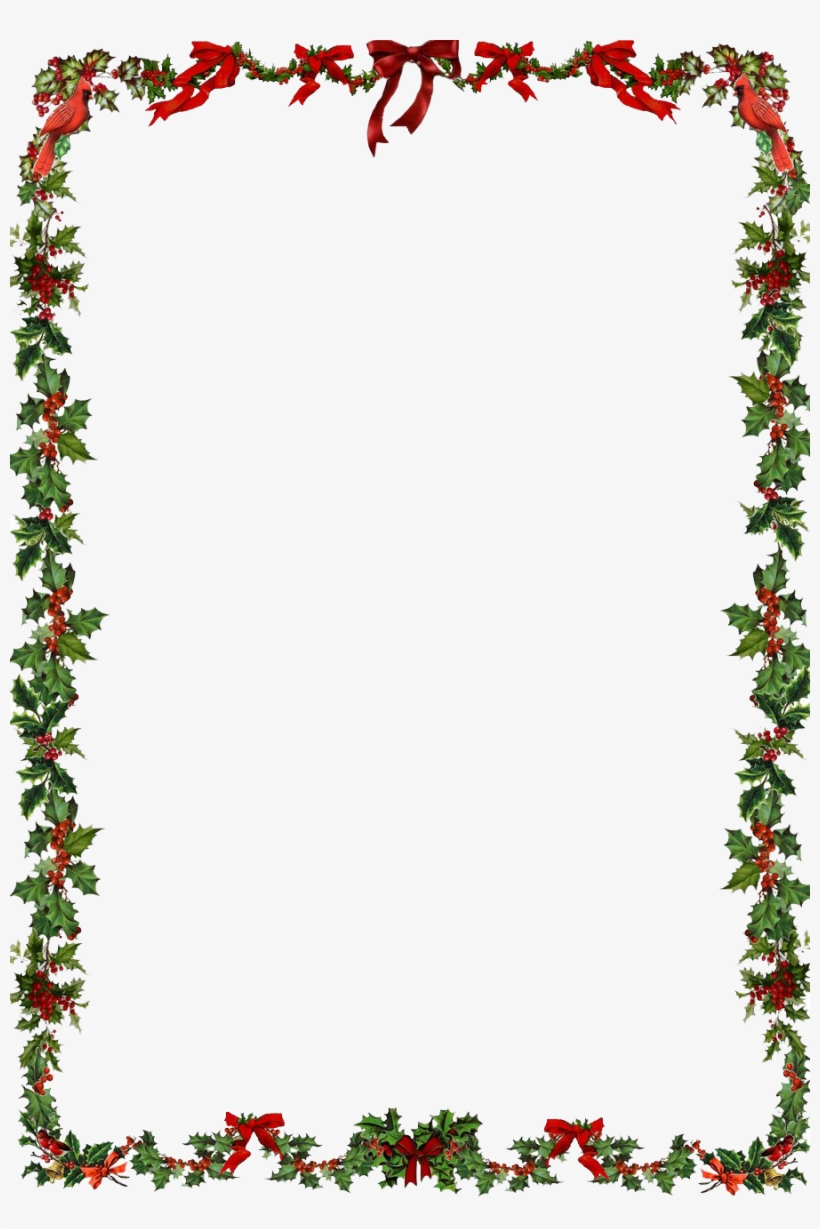
\includegraphics[width=\paperwidth,height=\paperheight]{images/XmasHollyA4frame.png}}%
}

\newcommand\numberthis{\addtocounter{equation}{1}\tag{\theequation}}

\newtcolorbox{MyOuterBox}{%
  enhanced,
  watermark graphics=images/santa_faces_watermark.jpg,
  watermark opacity=0.8,
  watermark zoom=2.0,
  breakable,
  frame style=JISpurple,
  colback=JISivory,
  colframe=JISpurple,
  title={
\includegraphics[width=0.9cm,height=0.9cm]{images/JIS Final Logo FA-02.png}\raisebox{3mm}{\Large{Christmas Maths Challenge}\hspace{16em} \Large{\bfseries\sffamily 14}}},
}

\newtcolorbox{MyInnerBox}[2][]{enhanced,%empty,
coltitle=JISpurple,colback=white,
breakable,
fonttitle=\bfseries\sffamily,
attach boxed title to top left={yshift=-1.5mm},
boxed title style={empty, size=small, top=1mm, bottom=0pt},
varwidth boxed title=0.5\linewidth,
frame code={
  \path (title.east|-frame.north) coordinate (aux);
\path[draw=JISpurple, line width=0.5mm, rounded corners,fill=white]
(frame.west) |- ([xshift=-2.5mm]title.north east) to[out=0, in=180] ([xshift=7.5mm]aux)-|(frame.east)|-(frame.south)-|cycle;
},
title={#2},#1}

\newtcolorbox{MyInnerSplitBox}[2][]{enhanced,%empty,
bicolor,sidebyside,sidebyside align=top seam,
righthand width=6.5cm,colbacklower=white,
sidebyside gap=5mm,
breakable,
coltitle=JISpurple,colback=white,
fonttitle=\bfseries\sffamily,
attach boxed title to top left={yshift=-1.5mm},
boxed title style={empty, size=small, top=1mm, bottom=0pt},
varwidth boxed title=0.5\linewidth,
frame code={
  \path (title.east|-frame.north) coordinate (aux);
\path[draw=JISpurple, line width=0.5mm, rounded corners,fill=white]
(frame.west) |- ([xshift=-2.5mm]title.north east) to[out=0, in=180] ([xshift=7.5mm]aux)-|(frame.east)|-(frame.south)-|cycle;
},
title={#2},#1}


\newtcolorbox{MySolutionBox}[1][]{%
  enhanced,
  breakable,
  frame style=JISpurple,
  colback=PaleGreen, colframe=green,
  title={\Large Solution},
  drop fuzzy shadow,
  halign=left,
  #1
}

%%%%%%%%%%%%%%%%%%%%%%%%%%%%%%%%%%%%%%%%%%%%%%%%%%
\newtoggle{SOLUTION}
%%% Uncomment the appropriate line below to show solutions %%%
% \toggletrue{SOLUTION}
\togglefalse{SOLUTION}
%%%%%%%%%%%%%%%%%%%%%%%%%%%%%%%%%%%%%%%%%%%%%%%%%


%%%%%%%%%%%%%%%%%%%%%%%%%%%%%%%%%%%%%%%%%%%%%%%%%%
%%%%%%            DOCUMENT BEGINS           %%%%%%
%%%%%%%%%%%%%%%%%%%%%%%%%%%%%%%%%%%%%%%%%%%%%%%%%%
\begin{document}


  \begin{MyOuterBox}
    \iftoggle{SOLUTION}{Here are the full, or partial solutions.
    }{
      Welcome to the Christmas Holiday Maths Challenge!\\
      Have a go at both questions!\\
      Drop your solution in the box in the staffroom next term.
    }
       \begin{MyInnerBox}{Year 8 and below}
     \begin{minipage}[t]{0.4\linewidth}
       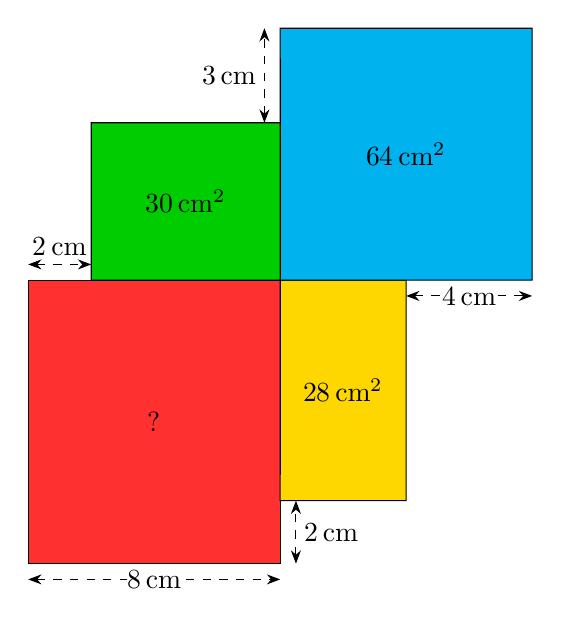
\begin{tikzpicture}[scale=0.4]
         \filldraw[black,fill=Firebrick1] (0,0) coordinate (A) -- (8,0) coordinate (B) -- (8,9) coordinate (C) -- (0,9) coordinate (D) -- cycle;
         \filldraw[black,fill=Gold1] (8,2) coordinate (E) -- (12,2) coordinate (F) -- (12,9) coordinate (G) -- (C) -- cycle;
         \filldraw[black,fill=DeepSkyBlue2] (C) -- (16,9) coordinate (H) -- (16,17) coordinate (I) -- (8,17) coordinate (J) -- cycle;
         \filldraw[black,fill=Green3] (C) -- (8,14) coordinate (K) -- (2,14) coordinate (L) -- (2,9) coordinate (M) -- cycle;
         \draw[dashed,Stealth-Stealth] (0,-0.5) -- (8,-0.5) node[midway,fill=white,inner sep=0pt] {\(\SI{8}{\cm}\)};
         \draw[dashed,Stealth-Stealth] (0,9.5) -- (2,9.5) node[midway,above=1mm,inner sep=0pt] {\(\SI{2}{\cm}\)};
         \draw[dashed,Stealth-Stealth] (12,8.5) -- (16,8.5) node[midway,fill=white,inner sep=0pt] {\(\SI{4}{\cm}\)};
         \draw[dashed,Stealth-Stealth] (8.5,0) -- (8.5,2) node[midway,right=1.0mm,fill=white,inner sep=0pt] {\(\SI{2}{\cm}\)};
         \draw[dashed,Stealth-Stealth] (7.5,14) -- (7.5,17) node[midway,left=1.0mm,fill=white,inner sep=0pt] {\(\SI{3}{\cm}\)};
         \node (N) at (4,4.5) {\(?\)};
         \node (O) at (5,11.5) {\(\SI{30}{\square\cm}\)};
         \node (P) at (10,5.5) {\(\SI{28}{\square\cm}\)};
         \node (Q) at (12,13) {\(\SI{64}{\square\cm}\)};
       \end{tikzpicture}\par
       Puzzle A
     \end{minipage}%
     \hfill
     \begin{minipage}[t]{0.5\linewidth}
       \hfill
       \begin{tikzpicture}[scale=0.4]
         \draw[black,fill=SlateBlue4] (0,0) coordinate (A) -- ({1+25/9},0) coordinate (B) -- ({1+25/9},9) coordinate (C) -- (0,9) coordinate (D) -- cycle;
         \draw[black,fill=Plum1] (B) -- ({7+25/9},0) coordinate (E) -- ({7+25/9},6) coordinate (F) -- ({1+25/9},6) coordinate (G) -- cycle;
         \draw[black,fill=OrangeRed4] (G) -- (F) -- ({7+25/9},9) coordinate (H) -- (C) -- cycle;
         \draw[black,fill=Yellow1] (D) -- (H) -- ({7+25/9},18) coordinate (I) -- (0,18) -- cycle;
         \draw[black,fill=Magenta3] (E) -- ({8+25/9+10/3},0) coordinate (J) -- ({8+25/9+10/3},6) coordinate (K) --(F) -- cycle;
         \draw[black,fill=OliveDrab1] (F) -- (K) -- ({8+25/9+10/3},18) coordinate (L) -- (I) -- cycle;
         \node[white] (M) at (1.8,3.5) {\(?\)};
         \node[] (N) at (6.8,3.5) {\(\SI{30}{\square\cm}\)};
         \node[white] (O) at (12,3.5) {\(\SI{20}{\square\cm}\)};
         \node[white] (P) at (6.8,7.5) {\(\SI{15}{\square\cm}\)};
         \node[] (Q) at (4.7,13.5) {\(\SI{70}{\square\cm}\)};
         \node[] (R) at (12,13.5) {\(\SI{40}{\square\cm}\)};
         \iftoggle{SOLUTION}{
           \node[white] (S) at (9.4,7.5) {\(b\)};
           \node[] (T) at (9.2,3.5) {\(2b\)};
           \node[] (U) at (14.7,3.5) {\(2b\)};
           \node[] (V) at (14.7,13.5) {\(4b\)};
         }{}
       \end{tikzpicture}\par
       Puzzle B\par
     \end{minipage}\par\medskip
     Two puzzles! Remember you have to show how you got the answer. You cannot justify your answer by saying "Because it looks that way!" Have fun!\par
     \iftoggle{SOLUTION}{%conditional output begin
      \begin{MySolutionBox}
        Puzzle A\par
        First we can see that the green-red boundary must be \(8-2=\SI{6}{\cm}\).\par
        Then, since the green rectangle is \(\SI{30}{\square\cm}\), the green-blue boundary has to be \(\SI{5}{\cm}\)\par
        Then, the height of the blue rectangle is \(\SI{8}{\cm}\) and so its width must be \(\SI{8}{\cm}\) too.\par
        Now, the width of the yellow rectangle must be \(8-4=\SI{4}{\cm}\) and so its height must be \(\SI{7}{\cm}\).\par
        From this we get the height of the red rectangle is \(7+2=\SI{9}{\cm}\).\par
        So the area of the red rectangle is \(8\times 9 = \SI{72}{\square\cm}\).\par\smallskip
        Puzzle B\par
        It is tempting to say the height of the pink rectangle plus the height of the dark red rectangle is the same as the yellow rectangle, which makes the unknown rectangle's area easy to find. But if that is true, we must \underline{show} it to be true.\par
        We let the height of the dark red rectangle be \(b\).\par
        Then the height of the pink rectangle must be \(2b\) as it has the same width but is double the area of the dark red rectangle.\par
        Now label the height of the purple rectangle \(2b\) as it is the same height as the pink rectangle, and the height of the light green rectangle \(2d\) as it has the same width as the purple rectangle but is double the area.\par
        But now we have shown that the height of the yellow rectangle is \(3b\), that is, we know that the yellow rectangle has the same area as the dark blue, dark red and pink rectangles put together.\par
        Therefore the area of the dark blue rectangle must be \(70-(15+30)=\SI{25}{\square\cm}\).\par
      \end{MySolutionBox}
    }{}%conditional output end
    \end{MyInnerBox}


    \vspace{0.4cm}
          \begin{MyInnerSplitBox}{Year 9 and above}
        The lengths of the sides of the three squares are consecutive integers. Find the area covered by the three squares.\par
      \iftoggle{SOLUTION}{%conditional output begin
      \begin{MySolutionBox}
        Let's call the length of the side of the smallest square \(a\).\par
        We can then write some of the other dimensions in terms of \(a\), and find the dimensions of the rectangular overlap of the larger two squares.\par
        Triangles \(\bigtriangleup ABC\) and \(\bigtriangleup ADE\) are congruent so \(ED=2\).\par
        Applying Pythagoras' Thm. to \(\bigtriangleup BDF\) we have,\par
        \begin{align*}
          4^{2} + (2a+2)^{2} &= (4\sqrt{10})^{2}\\
          4a^2 + 8a + 4 &= 160\\
          4a^{2} + 8a + 20 - 160 &= 0\\
          a^{2} + 2a - 35 &= 0\\
          (a+7)(a-5) &= 0
        \end{align*}
        Distance must be positive, so we reject the \(a=-7\) solution, and take \(a=5\).\par
        Now the total area is,
        \begin{align*}
          5^{2} + (5+1)^{2} + (5+2)^{2} &= 25 + 36 + 49\\
                                        &= 110\\
          \shortintertext{minus the overlapping rectangle,}
          110 - 2\times 1 &= \SI{108}{\square\cm}
        \end{align*}
      \end{MySolutionBox}
    }{}%conditional output end
        \tcblower
        \begin{tikzpicture}[scale=0.6]
          \draw[black,thick,fill=RosyBrown1] (0,0) coordinate (A) -- (6,0) coordinate (B) -- (6,6) coordinate (C) -- (0,6) coordinate (D) -- cycle;
          \draw[black,thick,fill=PaleTurquoise1] (B) -- (11,0) coordinate (E) -- (11,5) coordinate (F) -- (6,5) coordinate (G) -- cycle;
          \draw[black,thick,fill=NavajoWhite1,opacity=0.4] (4,5) coordinate (H) -- (F) -- (11,12) coordinate (I) -- (4,12) coordinate (J) -- cycle;
          \draw[Stealth-Stealth,Tomato4] (8,0) -- (J) node[pos=0.7,right] {\(4\sqrt{10}\)};
          \draw[dashed] (H) -- (4,0);
          \iftoggle{SOLUTION}{
            \node[below] (M) at (8.5,0) {\(a\)};
            \node[below] (N) at (2.5,0) {\(a+1\)};
            \node[above] (O) at (7.5,12) {\(a+2\)};
            \node[above] (P) at (2,6) {\(a-1\)};
            \node[below] (Q) at (5,5) {\(2\)};
            \node[left] (R) at (4,5.5) {\(1\)};
            \node[above right] at (C) {\(A\)};
            \node[above] at (J) {\(B\)};
            \node[below] at (7.7,0) {\(D\)};
            \node[above right] at (4,6) {\(C\)};
            \node[below] at (B) {\(E\)};
            \node[below] at (4,0) {\(F\)};
            \draw[dashed,Stealth-Stealth] (3.3,6) -- (3.3,12) node[midway,fill=white,inner sep=0mm] {\(a+1\)};
          }{}
        \end{tikzpicture}
    \end{MyInnerSplitBox}


  \end{MyOuterBox}

%%%%%%%%%%%%%%%%%%%%%%%%%%%%%%%%%%%%%%%%%%%%%%%%%%
\end{document}



